\documentclass{article} % For LaTeX2e
\usepackage{nips15submit_e,times}
\usepackage{hyperref}
\usepackage{url}
%\documentstyle[nips14submit_09,times,art10]{article} % For LaTeX 2.09
\usepackage{graphicx} % more modern
%\usepackage{epsfig} % less modern
%\usepackage{subfigure} 

\usepackage{amsmath}
\usepackage{amsfonts}
\usepackage{amsthm}
\usepackage{caption}
\usepackage{subcaption}

% For citations
\usepackage{natbib}

\usepackage{dsfont}

\usepackage{caption}
\DeclareCaptionType{copyrightbox}
\usepackage{subcaption}

\newcommand{\ones}{\ensuremath{\mathds{1}}}
\newcommand{\R}{\ensuremath{\mathds{R}}}
\newcommand{\veps}{\boldsymbol{\epsilon}}
\newcommand{\va}{\boldsymbol{\alpha}}
\newcommand{\Bw}{\mathbf{w}}
\newcommand{\Bx}{\mathbf{x}}
\newcommand{\By}{\mathbf{y}}
\newcommand{\Bg}{\mathbf{g}}
\newcommand{\BX}{\mathbf{X}}
\newcommand{\BK}{\mathbf{K}}
\renewcommand{\vec}[1]{\mathbf{#1}}

\newcommand{\felix}[1]{\textcolor{blue}{{\bf Felix:} #1}}
\newcommand{\nikolaas}[1]{\textcolor{green}{{\bf Nikolaas:} #1}}
\newcommand{\sebastian}[1]{\textcolor{red}{{\bf Sebastian:} #1}}

% For algorithms
\usepackage{algorithm}
\usepackage{algorithmic}

% As of 2011, we use the hyperref package to produce hyperlinks in the
% resulting PDF.  If this breaks your system, please commend out the
% following usepackage line and replace \usepackage{icml2016} with
% \usepackage[nohyperref]{icml2016} above.
\usepackage{hyperref}

% Packages hyperref and algorithmic misbehave sometimes.  We can fix
% this with the following command.



\title{Doubly stochastic large scale kernel learning \\ with the empirical kernel map}


\author{
Nikolaas Steenbergen\\
DFKI, Berlin, Germany\\
\texttt{nikolaas.steenbergen@dfki.de}\\
\And
Sebastian Schelter\\
TU Berlin, Berlin, Germany\\
\texttt{sebastian.schelter@tu-berlin.de}\\
\And
Felix Biessmann
TU Berlin, Berlin, Germany\\
\texttt{felix.biessmann@tu-berlin}\\
}

% The \author macro works with any number of authors. There are two commands
% used to separate the names and addresses of multiple authors: \And and \AND.
%
% Using \And between authors leaves it to \LaTeX{} to determine where to break
% the lines. Using \AND forces a linebreak at that point. So, if \LaTeX{}
% puts 3 of 4 authors names on the first line, and the last on the second
% line, try using \AND instead of \And before the third author name.

\newcommand{\fix}{\marginpar{FIX}}
\newcommand{\new}{\marginpar{NEW}}

%\nipsfinalcopy % Uncomment for camera-ready version

\begin{document}


\maketitle

\begin{abstract} 
With the rise of big data sets the popularity of kernel methods declined and neural networks took over again. The reason kernel methods have become unpopular is that the kernel matrix grows quadratically with the number of data points. Most attempts to scale up kernel methods  solve this problem by discarding data points or basis functions of some approximation of the kernel function. Here we present a simple yet effective way of scaling up kernel methods via doubly stochastic optimization of the emprical kernel map. We build our work on a large body of existing theoretical work on kernel machines and provide empirical evidence that the algorithm works in practice on large data sets and can leverage the full power and versatility of classical kernel machines. Most importantly the algorithm is simple to implement, especially in settings using parallel execution.
\end{abstract} 


\section{Introduction\vspace{-0.1in}}
\indent When kernel methods \cite{Muller:2001p2592,learning_with_kernels,shawe2004kernel} were introduced in the machine learning community, they quickly gained popularity and became the gold standard in many applications. One reason for this was that kernel methods are powerful tools for modelling non-linear dependencies. Even more importantly, kernel methods offer a convenient split between modelling the data with an expressive set of versatile kernel functions for all kinds of data types (e.g., graph data \cite{shawe2004kernel} or text data \cite{John2000}), and the learning part, including both the learning paradigm (unsupervised vs. supervised) and the optimization. 

The main drawback of kernel methods is that one needs to compute the kernel matrix $\vec{K}\in\R^{N\times N}$, where $N$ is the number of samples. For large data sets this kernel matrix can neither be computed nor stored in memory. Even worse, the learning part of kernel machines often has complexity $\mathcal{O}(N^3)$. This renders standard formulations of kernel methods intractable for large data sets. When machine learning entered the era of web-scale data sets, artificial neural networks, enjoying learning complexities of $\mathcal{O}(N)$, took over again and have been dominating the top ranks of competitions, the press on machine learning and all major conferences since then. But the advantage of neural networks -- or other non-linear supervised algorithms that perform well on large data sets in many applications, such as Random Forests \cite{Breiman2001} -- leaves many researchers with one question (see e.g. \cite{Lu2014}): What if kernel methods could be trained on the same amounts of data that neural networks can be trained on? 

There have been several attempts to scale up kernel machines, most of which fall into two main categories: a) approximations of the kernel map based on subsampling of Fourier basis functions (see \cite{Rahimi2008}) or b) approximations of the kernel matrix based on subsampling of data points (see \cite{Williams2000}).
%
While both of these are powerful methods and often achieve competitive performance, most applications of these approximations solve the problem of scaling up kernel machines by discarding data points or Fourier basis functions from the computationally expensive part of the learning. 
Here we present a remarkably simple yet effective way of scaling up kernel methods that -- in contrast to many previous approaches -- can make use of the entire data set. 

Similar to \cite{Dai2014}, we propose a doubly stochastic approximation to scale up kernel methods. In contrast to their work however, who use the {\em explicit} kernel map\footnote{We follow the convention that {\em explicit} kernel maps refer to a data independent kernel map approximation, see also \autoref{sec:kernels}.}, we propose to use the empirical kernel map. While the optimization follows a similar schema, there is evidence suggesting that approximations of the explicit kernel map can result in lower performance \cite{Yang2012}.

The approach is called doubly stochastic because there are two sources of noise in the optimization: a) the first source samples random data points at which a noisy gradient of the dual coefficients is evaluated and b) the second source samples data points at which a noisy version of the empirical kernel map is evaluated. We propose a redundant data distribution scheme that allows for computing approximations that go beyond the block-diagonal of the full kernel matrix, as proposed e.g. in \cite{Deisenroth2015}. We perform experiments on synthetic data comparing the proposed approach with other approximations of the kernel map, and conduct experiments with a parallel implementation to show the scale-up behaviour on a large data set. 

In the following, we give a short summary of the essentials on kernel machines, in \autoref{sec:large_scale_kernel_learning} we give a broad overview over some attempts to scale up kernel methods, \autoref{sec:dskl} outlines the main idea of the paper and \autoref{sec:experiments} contains our experiments.

\section{Kernel methods recap}\label{sec:kernels}
This section summarizes some of the essentials of kernel machines. For the sake of presentation we only consider supervised learning and assume $D$-dimensional real-valued input data $\Bx_i\in\R^D$ and a corresponding boolean label $y_i\in\{-1,1\}$. Extensions to multivariate real valued labels or unsupervised learning methods are possible, as in e.g.  \cite{Lopez-Paz2014}. At the heart of kernel machines is the so-called {\em kernel trick}: The function to be learned function $\phi^*(\Bx_i) $ (evaluated at the $i$th data point $\Bx_i$) is modelled as a linear combination $\va\in\R^N$ of similarities among data points mapped to a (potentially infinite dimensional) {\em kernel feature space} $\mathcal{S}$

\begin{align}\label{eq:kernel_trick}
\phi^*(\Bx_i)=\sum_{j=1}^N k(\Bx_i,\Bx_j)\alpha_j.
\end{align}
Here $N$ again denotes the number of data points in a data set, $\alpha_i$ denotes the $i$th entry of $\va$, and the kernel function $k(.,.)$ measures the similarity of data points in the kernel feature space by computing inner products in $\mathcal{S}$
\begin{align}\label{eq:kernel_function}
k(\Bx_i,\Bx_j)=\langle \phi(\Bx_i), \phi(\Bx_i)\rangle_{\mathcal{S}}.
\end{align}
%
Taking the shortcut through $k(.,.)$, i.e. mapping data points to $\mathcal{S}$ and computing their inner products without ever formulating the mapping $\phi$ {\em explicitely} when learning $\phi$ is sometimes called {\em kernel trick}. Methods that attempt to construct an {\em explicit} representation of $\phi$ are hence sometimes referred to as {\em explicit kernel approximations}, see e.g. \cite{Dai2014}. 

Most kernel machines then minimize a function $\mathcal{E}(y, \Bx, \va, k)$ which combines a loss function $l(y, \Bx, \va, k)$ with a regularization term $r(\va)$ that controls the complexity of $\phi$ 
%
\begin{align}\label{eq:error_function}
\mathcal{E}(y, \Bx, \va, k) = r(\va) + l(y, \Bx, \va, k).
\end{align}
%
The regularizer $r(\va)$ often takes the form of some $\mathcal{L}_p$ norm of the vector of dual coefficients $\va$, where usually $p=2$. A popular example of \autoref{eq:error_function} is that of the kernel support-vector machine (SVM) \cite{Cortes1995}, a hinge los combined with a quadratic regularizer
%
\begin{equation}\label{eq:svm_gradient}
\mathcal{E}_{SVM} = ||\max \left(0,\ones-\text{diag}(\vec{y}) \vec{K} \va \right)||_1 + \lambda ||\va||_2, \quad \frac{\mathcal{E}_{SVM}}{\partial \va} =\max \left(0,1-\left(\lambda\va - \vec{y}^{\top}\vec{K}\right)\right).
\end{equation}
%
Other examples of popular kernel methods include a least squares loss function combined with $\mathcal{L}_2$ regularization, also known as Kernel Ridge Regression, Kriging \cite{kriging} or the mean function of Gaussian Processes, and spectral decompositions of the kernel matrix such as kernel PCA \cite{Scholkopf:1998p427}. We refer the interested reader to \cite{learning_with_kernels,shawe2004kernel} for an overview. 

\subsection{Large Scale Kernel Learning}\label{sec:large_scale_kernel_learning}
Evaluating the empirical kernel map in \autoref{eq:kernel_function} for one data point comes at the cost of $N$ evaluations of the kernel function, since the index $j$ (which picks the data points that are used for expanding the {\em kernel map}) runs over all data points in the data set\footnote{Actually the complexity is of $\mathcal{O}(ND)$ where $D$ is the dimensionality of the data, but as this is constant given a data set, we omit this factor here.} both for training and predicting. Computing the full gradient with respect to $\va$ requires $N$ evaluations, too, so the total complexity of computing the gradient of a kernel machine is in the order of $\mathcal{O}(N^2)$. This is the reason why kernel methods became unattractive for large data sets -- other methods like linear models or neural networks can be trained in $\mathcal{O}(N)$ time. 

One can categorize attempts to scale up kernel methods into two classes: a) Reducing the number of data points when evaluating the empirical kernel map in \autoref{eq:kernel_function} and b) avoiding to evaluate the empirical kernel map altogether by using an {\em explicit approximation} of the kernel map. There are more sophisticated approaches within each of these categories that can give a quite significant speedup \cite{Le2013, Rudi2015}. Here we focus on a comparison between these two types of approximations. We emphasize however that many of these additional improvements also apply to the approach proposed in this manuscript and are likely to improve convergence and runtime. In the following, we briefly survey some research in both categories.

\paragraph{Empirical / Implicit kernel maps:} The first approach, reducing the number of data points when evaluating the kernel function, amounts to subsampling data points for computing the empirical kernel map in \autoref{eq:kernel_function}. 
The data points used to compute the empirical kernel map are sometimes referred to as {\em landmarks} \cite{Hsieh2014}. 
A prominent line of research in this direction follows what is commonly referred to as the {\em Nystr\"om method} \cite{Williams2000}. The key idea here is that instead of using the entire kernel matrix one can take a low-rank approximation of that matrix computed on a randomly subsampled part of the data. 
Other in this direction aims at sparsifying the vector of dual coefficients $\va$, see e.g. \cite{WilsonN15, LiangP15}. 
There are two main problems with these approaches. For one, a large number of data points is discarded. Even if this is done with some smart selection criteria, these are usually not computed in kernel feature space; thus this procedure can have detrimental effects on the final performance. Second many of these methods are difficult to implement, especially in a distributed setting. In general, applying kernel methods in distributed settings is challenging. One approach is to simply distribute the data to different workers and solve the kernel problems independently on each worker \cite{Deisenroth2015}. This implicitly assumes that the kernel matrix is a block diagonal matrix where the blocks on the diagonal are the kernels on each worker -- all the rest of the kernel matrix is neglected.

\paragraph{Explicit kernel maps:} Recent approaches for large scale kernel learning avoid computation of the kernel matrix by relying on {\em explicit} forms of the kernel function \cite{Rahimi2008,Vedaldi2010}. The basic idea is that instead of using a kernel function $k$, which {\em implicitly} projects the data to kernel feature space $\mathcal{S}$ and computes the inner products in that space in one step, {\em explicit} kernel functions just perform the first step, mapping to kernel feature space with an approximation of the kernel map $\phi(.)$. This has the advantage that the effective number of features can be controlled directly. The model then learns simply a linear combination of these features. Explicit feature maps often express the kernel function as a set of Fourier basis functions. A comprehensive overview of kernel functions and their explicit representations can be found in \cite{Dai2014}. A more detailed explanation with graphical illustrations for a small set of kernel functions can be found in \cite{Vedaldi2010}. In the context of large-scale kernel learning this method was popularized by Rahimi and Recht under the name of {\em random kitchen sinks} \cite{Rahimi2008}. An important parameter choice in these approaches is the number of basis functions. This choice determines the accuracy of the approximation as well as the speed of the computations. 

\paragraph{Which approximation is better?}
Both approaches, {\em implicit kernel maps} and {\em explicit kernel maps}, are similar in that they approximate a potentially infinite dimensional space $\mathcal{S}$. The main difference is that for empirical kernel map approaches, the approximation samples data points (and in most cases simply {\em discards} a lot of data points), while in the case of explicit kernel map approximations the approximation samples random Fourier basis functions. In practice there are many limitations on how much data can be acquired and how much data can be processed efficiently. The type of data can also make a difference in the performance of either approximation: When using the empirical kernel map on extremely sparse data, the empirical kernel function evaluated on a small subset of data points will return 0 in most cases -- while Fourier bases with low frequencies will cover the space of the data much better. 

Which of the two approximations is better in practice is likely to depend on the data. 
Some empirical evidence suggests that the Nystr\"om approximation is better than random kitchen sinks \cite{Yang2012}. The authors of \cite{Vedaldi2010} perform an extensive comparison of various explicit kernel map approximations and empirical kernel maps, highlighting the advantages in the empirical kernel map approach: Empirical kernel maps have the potential to model some parts of the input distribution better -- but they have to be trained on data; this can be considered as a disadvantage. But then again any machine learning algorithm has to learn from data. There could be scenarios in which learning the feature representation (via empirical kernel maps) along the way gives performance gains. We are not aware of a concise comparison of the two approaches in a parallel setting. In our experimental section we provide a direct comparison between the two methods keeping the optimization part fixed and concentrating on the type of approximation. 
%
\section{Doubly stochastic kernel learning}\label{sec:dskl}
This section describes the learning approach, which follows the pseudocode sketched in Algorithm \autoref{alg:dskl} for a pair of data points. The idea is that in each iteration a random sample $\mathcal{I}\subseteq\{1,2,\dots,N\}, |\mathcal{I}|=I$ of data points is chosen for computing the gradient of the dual coefficients $\va$ and another (independent) random sample  $\mathcal{J}\subseteq\{1,2,\dots,N\}, |\mathcal{J}|=J$ of data points is chosen for expanding the empirical kernel map $k(.,.)$. Note that this is very similar to Algorithm 1 and 2 in \cite{Dai2014}, except that instead of drawing random basis functions of the kernel function approximation, we sample random data points. If one were to compute the entire kernel matrix $\vec{K}\in\R^{N\times N}$, this procedure would correspond to sampling a rectangular submatrix $\vec{K}_{\mathcal{I,J}}\in\R^{I\times J}$. The number of data points sampled for expanding the empirical kernel map as well as the number of data points to compute the gradient are important parameters that determine the noise of the gradient of the dual coefficients and the noise of the empirical kernel map, respectively. The pseudocode in algorithm \autoref{alg:dskl} summarises the entire procedure, which alternates two steps: 1) sample a random submatrix of the kernel matrix and 2) take a gradient step along the direction of $\frac{\partial\mathcal{E}}{\partial \va_{\mathcal{J}}}$.

% 
\begin{algorithm}
  \begin{algorithmic}
    \caption{Doubly Stochastic Kernel Learning\label{alg:dskl}}
     \REQUIRE $(\Bx_i,y_i),i\in\{1,\dots,N\},\Bx_i\in\R^{D},~y_i\in\{-1,+1\}$, Kernel $k(.,.)$
    \ENSURE Dual coefficients $\va$ 
   \STATE \# Initialize coefficients $\va$, initialize counter $i=0$
   \WHILE{Not Converged}
   \STATE $t\gets t+1$
   \STATE \# Sample indices $\mathcal{I}$ for gradient 
   \STATE $\mathcal{I}\sim\text{unif}(1,N)$
   \STATE \# Sample indices $\mathcal{J}$ for empirical kernel map
   \STATE $\mathcal{J}\sim\text{unif}(1,N)$
   \STATE \# Compute Gradient
   \STATE $\vec{g}_{\mathcal{J}} \gets \frac{\partial \mathcal{E}}{\partial\va_{\mathcal{J}}}$ (see e.g. \autoref{eq:svm_gradient})
   \STATE \# Update weight vector 
   \STATE $\forall j\in\mathcal{J}: \alpha_j\gets\alpha_j - 1/t~ g_j$ 
   \ENDWHILE
  \end{algorithmic}
\end{algorithm}
%
Note that in contrast to some other kernel approximations the memory footprint of this algorithm is rather low: While low-rank approximations need to store the low rank factors, algorithm \autoref{alg:dskl} requires only to store the dual coefficients $\va$. 
The learning rate parameter here is simply set to $1/t$ where $t$ is the number of iterations. It is good practice to adjust that parameter according to some more sophisticated schedule. We emphasize that many standard methods to speed up convergence of stochastic gradient, e.g. by better controlling the variance of the gradients can be applied.
%
\section{Experiments}\label{sec:experiments}
This experimental section describes experiments on artificial data and on publicly available real-world data sets. All experiments use a support-vector machine with RBF kernel, for the sake of comparability. We performed experiments on a single machine with serial execution as well as with a parallel shared-memory variant of our approach. We chose the batch SVM implementation available in scikit~learn~\cite{sklearn_api}. Experiments with serial execution were conducted for small-scale experiments, while we leverage the parallel variant for larger scale experiments. 

\paragraph{Hyperparameter optimization} Hyperparameters were tuned with two-fold cross-validation and exhaustive grid search for all models; the reported accuracies were computed on a held out test set of the same size as the training set. Hyperparameters for batch and SGD algorithms (the regularization parameter and RBF scale) were selected from a logarithmic grid from $10^{-6}-10^6$; The SGD approaches have additional parameters such as the step size (candidates were $10^{-4}-10^4$) and the minibatch size $I$ for computing the gradient. For doubly stochastic kernel learning and for random fourier features there is the additional hyperparameter $J$, referring to the number of kernel expansion coefficients or random fourier features, respectively.

\paragraph{Comparisons with related methods}
We compared the proposed method with other kernel approximations as well as with batch kernel SVMs. We conducted comparisons with random kitchen sinks (RKS) where the number of basis functions matched the number of expansion coefficients $J$. In order to assess standard large-scale kernel approximations that only use a subset of data points, we also compared with a version in which we first draw one random sample from the data, and then train the algorithm with that subset only. While most of these methods that use just a subset of the data apply more sophisticated schemes for selecting that subset and smarter ways of extrapolating, we wanted to focus on the main difference here, which is training on a fixed random subset of the data. 

\paragraph{Data sets}
In order to provide a qualitative comparison between the different kernel map approximations, we performed experiments on small synthetic data sets. We chose the XOR problem described in \autoref{fig:toy_data} as a benchmark for nonlinear classification. We also performed experiments on a number of standard benchmark real world data sets available on the libsvm homepage\footnote{\url{https://www.csie.ntu.edu.tw/~cjlin/libsvmtools/datasets/binary.html}}. The list of data sets can be found in \autoref{tab:small_realdata}. 
%
\begin{figure}[!ht]
    \centering
           \hfill
        \begin{subfigure}[b]{0.5\textwidth}
         Artificial data was generated for a standard two class nonlinear prediction benchmark, the XOR problem.
        Data for one class (yellow dots) is drawn from a spherical gaussian distribution $\mathcal{N}(0,0.2)$ around $[1,1]^\top$ and $[-1,-1]^\top$, and data points from the other class (red dots) are drawn from the same gaussian distribution centered around $[1,-1]^\top$ and $[-1,1]^\top$. 
         Background colors show the classification hyperplane learned by doubly stochastic SVM learning; support vectors are shown as larger circles.\\     
        \end{subfigure}
	\hfill
         \begin{subfigure}[b]{0.4\textwidth}
         \centering
        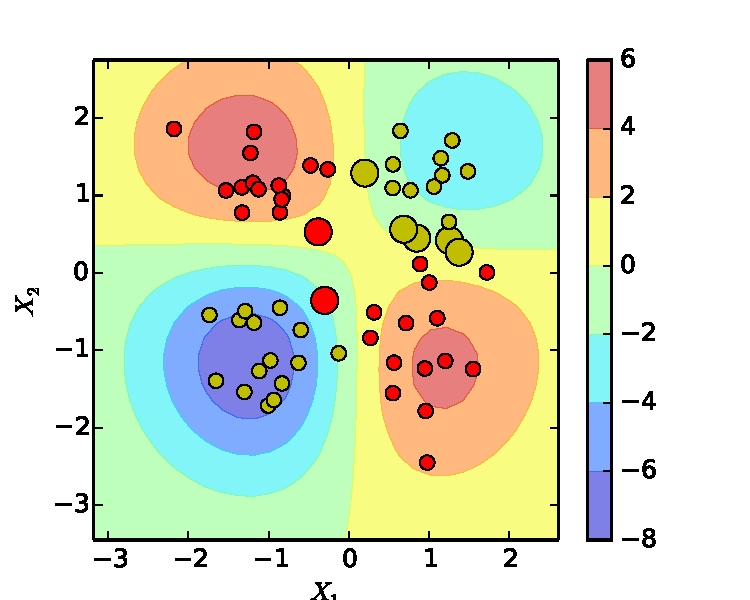
\includegraphics[width=1\columnwidth]{imgs/svm_kernel}
               \label{fig:toy_data}
        \end{subfigure}

        \caption{\label{fig:toy_data} Synthetic data generation for the XOR problem.}
\end{figure}


\subsection{Serial Execution}\label{sec:single_host}
We ran small-scale experiments in a single threaded implementation of algorithm~\autoref{alg:dskl}. We generated $N=100$ data points according to the XOR problem, see \autoref{fig:toy_data}, and optimized all hyperparameters as described in \autoref{sec:experiments}.
%
\autoref{fig:toydata_comparisons} shows comparisons of the proposed method with random kitchen sinks and a fixed random selection of data points, as well as with a batch setting. We plot the error on the test set when varying $I$, the number of samples for computing the gradient, in \autoref{fig:expand_20_pred_1} and \autoref{fig:expand_20_pred_50}. \autoref{fig:pred_20_expand_1} and \autoref{fig:pred_20_expand_50} show the error when varying $J$, the number of expansion coefficients. Note that with too few data points for computing the gradient or the expansion, both random kitchen sinks as well as a fixed sample of data points have an advantage over the doubly stochastic approach. As the number of data points in the gradient computation and the kernel map expansion increases however, doubly stochastic kernel learning achieves performance comparable to that of batch methods, indicated as dotted line.
%
\begin{figure}[!ht]
   \centering
    \begin{subfigure}[b]{0.235\textwidth}
        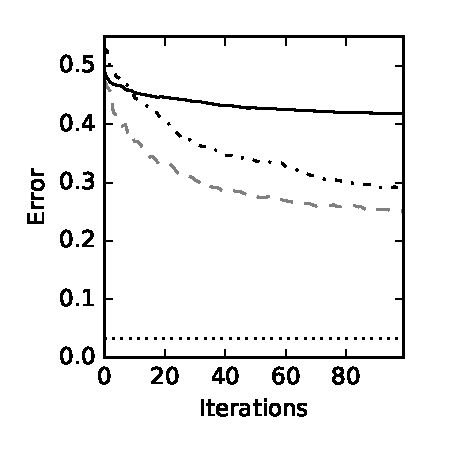
\includegraphics[width=\textwidth]{imgs/rks_emp_comparison-expand-20-pred-1}
        \caption{$I=1, J=20$}
        \label{fig:expand_20_pred_1}
    \end{subfigure}
    \hfill
    \begin{subfigure}[b]{0.235\textwidth}
        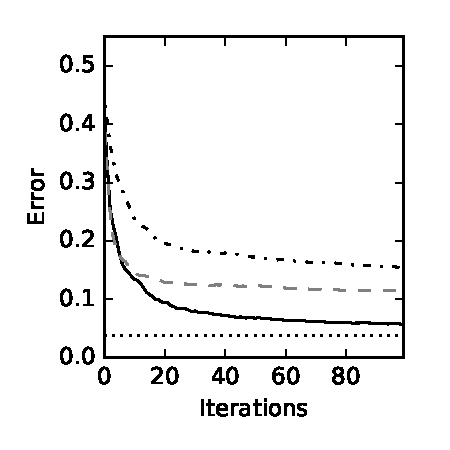
\includegraphics[width=\textwidth]{imgs/rks_emp_comparison-expand-20-pred-50}
        \caption{$I=50, J=20$}
        \label{fig:expand_20_pred_50}
    \end{subfigure}
        \begin{subfigure}[b]{0.235\textwidth}
        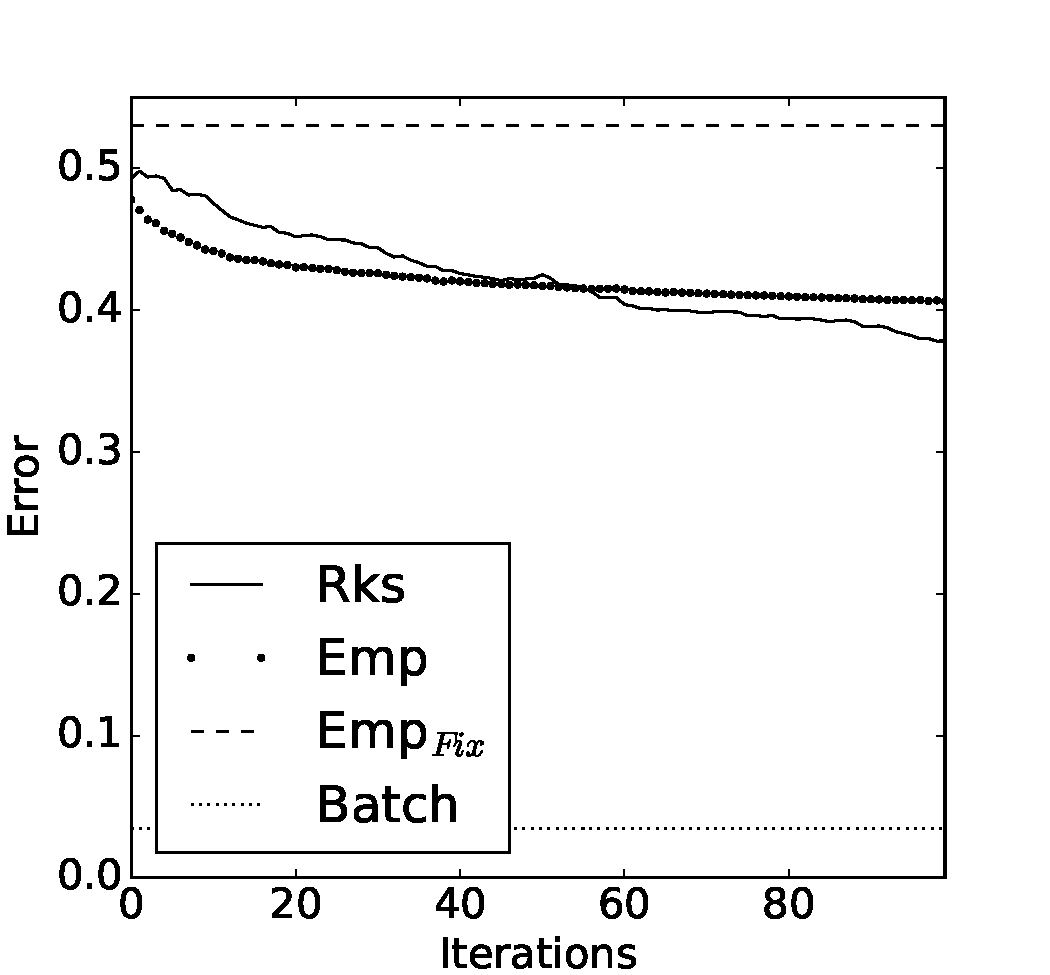
\includegraphics[width=\textwidth]{imgs/rks_emp_comparison-pred-20-expand-1}
        \caption{$I=20, J=1$}
        \label{fig:pred_20_expand_1}
    \end{subfigure}
    \hfill
    \begin{subfigure}[b]{0.235\textwidth}
        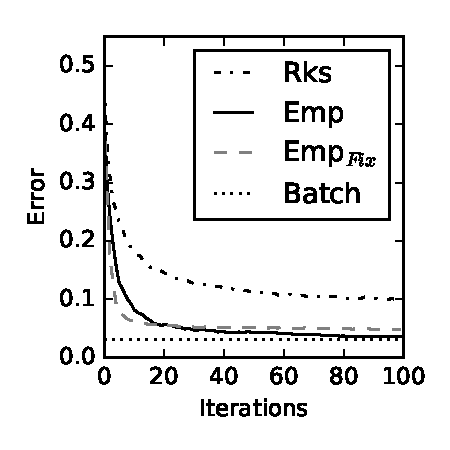
\includegraphics[width=\textwidth]{imgs/rks_emp_comparison-pred-20-expand-50}
        \caption{$I=20, J=50$}
        \label{fig:pred_20_expand_50}
    \end{subfigure}
    \caption{Error on test data for XOR problem in \autoref{fig:toy_data} for doubly stochastic kernel learning with the empirical kernel map (Emp), random kitchen sinks (RKS), random subsampling (Emp$_{\text{Fix}}$) and batch SVM}
    \label{fig:toydata_comparisons}
\end{figure}
%

We performed experiments on a number of standard benchmark real world data sets available on the libsvm homepage\footnote{\url{https://www.csie.ntu.edu.tw/~cjlin/libsvmtools/datasets/binary.html}}. We compare to the batch version using serial execution and small data sets. We discuss experiments on a larger dataset, leveraging our parallel variant in \autoref{sec:distributed}. For all experiments, we sampled $\min(1000,N_{\text{dataset}})$ data points where $N_{\text{dataset}}$ is the number of data points in the respective data set, and took half the data for training and half the data for testing, including hyperparameter optimization on the training set. We ran 10 repetitions of each experiment and show the test set error in \autoref{tab:small_realdata}. In all data sets  investigated, the proposed doubly stochastic empirical kernel learning approach achieves errors comparable to that of a batch SVM. In cases where the batch SVM achieves perfect accuracy and DSEKL still results in a few errors, we emphasize that we conduct these comparisons to show that DSEKL has the potential to achieve performance comparable to that of batch methods. Refining the SGD optimization or running more iterations could further improve the performance, yet our main intention is to only provide a proof of concept for the doubly stochastic approach. Also note that the proposed DSEKL approach only uses a fraction of the data in each step. This allows for training on much larger data sets, which we discuss in the next section.
%
\begin{table}
\begin{center}
\begin{tabular}{ ccc } 
Data Set & DSEKL & Batch\\
 \hline
MNIST small & 0.00$\pm$0.01  & 0.00$\pm$0.01\\
Diabetes & 0.20$\pm$0.02  & 0.22$\pm$0.02\\
Breast Cancer &  0.03$\pm$0.01 & 0.03$\pm$0.01\\
Mushrooms & 0.03$\pm$0.01 & 0.00$\pm$0.00\\
Sonar & 0.22$\pm$0.07 & 0.26$\pm$0.04\\
Skin/non-skin & 0.03$\pm$0.01 &  0.01$\pm$0.00\\
Madelon & 0.03$\pm$0.01 &  0.00$\pm$0.00\\
 \hline
\end{tabular}
\caption{Test error (mean $\pm$ standard deviation across 10 repetitions) on real world data sets. Doubly stochastic empirical kernel learning (DSEKL) achieves performance comparable to that of a batch kernel SVM. \label{tab:small_realdata}}
\end{center}
\end{table}
%
 \subsection{Parallel Execution using a Shared-Memory Variant}\label{sec:distributed}
This section describes the experiments performed using a parallel, shared-memory variant of our approach. We list the pseudocode in algorithm~\autoref{alg:dskl_svm_distributed}. The difference to algorithm~\autoref{alg:dskl} is that we run multiple workers at the same time, and process multiple samples for the empirical kernel map per iteration to parallelize learning. We use sampling without replacement to partition the data for the different workers. 

 \begin{algorithm}
   \begin{algorithmic}[1]
     \caption{Parallel Shared-Memory Nonlinear Support-Vector Machine\label{alg:dskl_svm_distributed}}
       \REQUIRE sample size $s$, number of workers $K$
       \STATE \# Initialize coefficients $\va$
       \STATE \# Sample indices $\mathcal{I}^{(0)},\dots,\mathcal{I}^{(K)}$ for gradient 
       \STATE \# Sample indices $\mathcal{J}^{(0)},\dots,\mathcal{J}^{(K)}$ for empirical kernel map 
       \STATE $\vec{G} \leftarrow \mathbb{I}$
       \WHILE{Not Converged}
         \FORALL{samples $\mathcal{I}^{(0)},\dots,\mathcal{I}^{(K)}$}      
           \FORALL{samples $\mathcal{J}^{(0)},\dots,\mathcal{J}^{(K)}$ in parallel on worker $k$} 
             \STATE \# Compute gradients as in Algorithm~\autoref{alg:dskl}
             \STATE $\vec{g}^{(k)} \gets \frac{\partial \mathcal{E}}{\partial\va}$
             \STATE \# Aggregate inverse gradients for dampening updates of $\va$
             \STATE $\vec{G}_{ii} \leftarrow \vec{G}_{ii} + \left(g^{(k)}_{ji}\right)^2$ for all $i \in\mathcal{I}^{(k)}$ and $j\in\mathcal{J}^{(k)}$
           \ENDFOR
         \ENDFOR
         \STATE \# Update weight vector 
         \STATE $\va \leftarrow \va - \vec{G}^{-\frac{1}{2}} \sum_k \vec{g}^{(k)}$
       \ENDWHILE
   \end{algorithmic}
 \end{algorithm}

\sebastian{we need to list the experiments of Nikolaas here}


\begin{figure}[!ht]
	\begin{subfigure}[b]{0.5\textwidth}
		\centering
		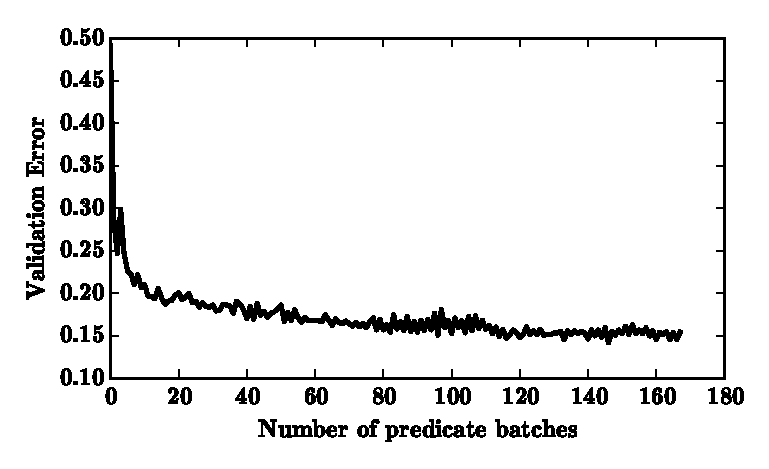
\includegraphics[width=\textwidth]{imgs/covertype_validation.pdf}
		\caption{Validation error per epoche on full Covertype Dataset}
		\label{fig:covertype_validation}
	\end{subfigure}
	\begin{subfigure}[b]{0.5\textwidth}
		\centering
		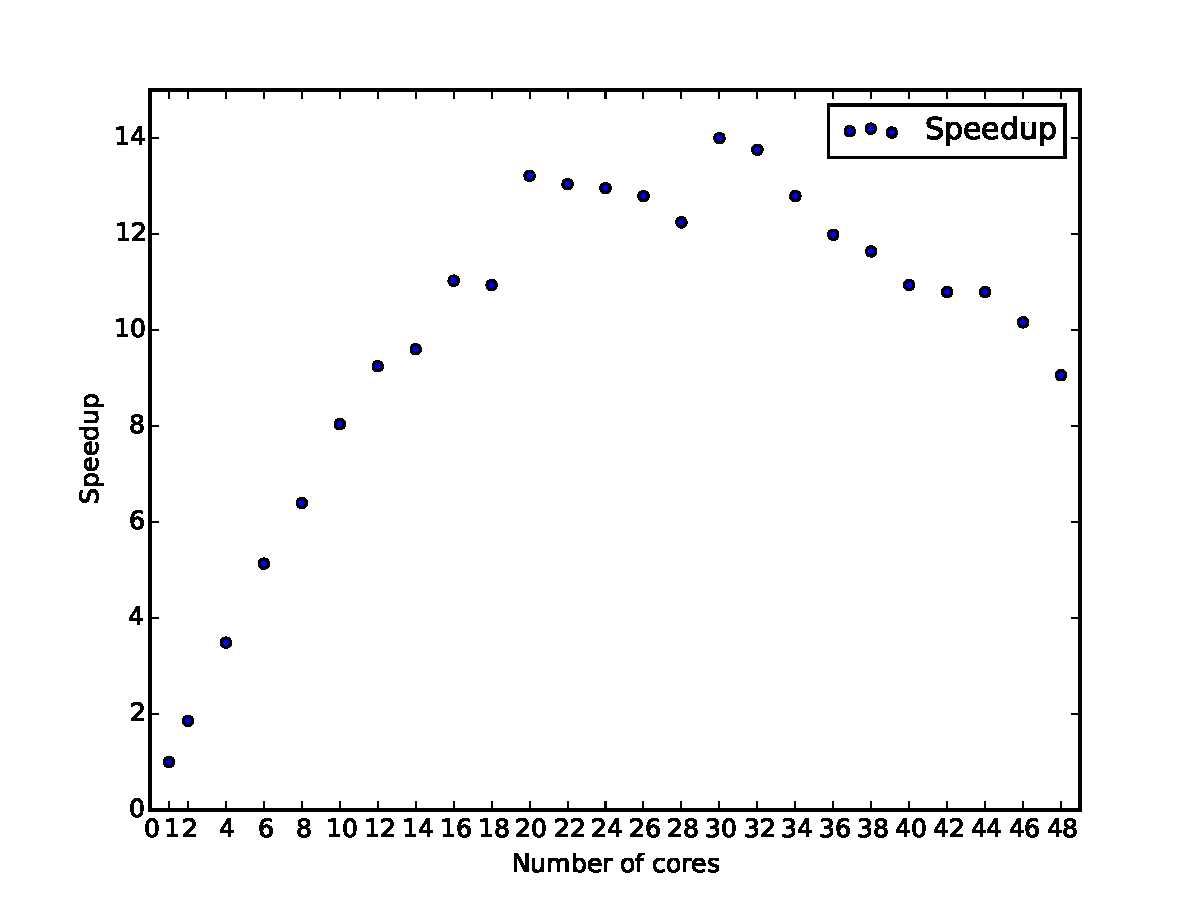
\includegraphics[width=\textwidth]{imgs/speedup_58.pdf}
		\caption{Speedup on a single machine with multiple cores. All speedups are compared to runtime on two cores.}
		\label{fig:speedup_58}
	\end{subfigure}
\end{figure}

We ran our experiment on the covertype dataset~\footnote{\url{https://archive.ics.uci.edu/ml/datasets/Covertype}}, consisting of ca 581,012 datapoints with 54 features. We drew samples of 10,000 points for training and 10,000 kernel samples (such that the samples still fit into main memory), and set the regularization parameter $C$ to $1 / N_{dataset}$, and fix the RBF scale to $1.0$. We employ a weight decay factor of $\frac{1}{i}$, where $i$ is the number of epochs. We stop the training process if the $L_{2}$ norm of the weight change over one epoch is less than $1$. Additionally, we separate 1122 random samples for validation after each training epoch (i.e.,~computing all gradients for all combinations of training point sample and kernel map sample).
Figure \ref{fig:covertype_validation} depicts the validation error after each epoch. Note, that after one epoch the validation error decreases drastically from 51\% to 17\%. We separated a random sample of 20,000 data points as test set from the training data. We achieve a final error rate on the test set of 13.34\%. 
These results are comparable to \cite{Dai2014}, which also achieve a test error of also about 17\% after one iteration. 
\nikolaas{Kann man das so sagen ? Die sagen ungefähr 15\%, im graphen ist das eher 17, wisst ihr sonst noch was man vergleichen könnte? }
\sebastian{wenn die 15 sagen, sollten wir ihnen das glauben :) Sind wir nach einer Epoch bei 13.34?}

Figure \ref{fig:speedup_58} shows the speedup achieved through the usage of multiple cores in a shared memory architecture.
A python implementation of our algorithm runs on a 48 core machine with 500 gb main memory. We measure the time of processing one training data batch, which is evaluated against all kernel batches in parallel on the full covertype dataset. This amounts to a degree of parallelism of 58 for one training batch evaluation. We measure speedups against the runtime on 2 cores \sebastian{wäre viel besser gegen einen core zu vergleichen, dann sind auch die zahlen groesser :)}, and increase by the parallelism by two cores at a time.

We observed a linear speedup until 20 cores where we achieved an 8 times speedup compared to only 2 cores. After that, the speedup curve flattens out, and finally drops after 32 cores. \sebastian{This needs to be rewritten, we need to be more sure here...}
A possible explanation for the drop in speedup using more than 30 cores could be the implementation of python process that are used for concurrent computations. The data is not shared but serialized and sent, when a new process is spawned, creating additional overhead with an increased number of processes.
%A possible explanation for the drop in speedup after 30 cores could be the Global interpreter lock (GIL) of python, which results in increased communication 
%\nikolaas{oder ``locking'' overhead, thread muss 10 mal anfragen ob er dran sein darf oder ob noch alles gelockt ist, so hab ich das verstanden..} overhead the more processes we spawn.
\sebastian{We need a summary here: We achieve comparable performance and show huge parallelization potential.}





% \subsection{Distributed infrastructure}\label{sec:distributed}
% This section describes the experiments performed on distributed infrastructure. We list the pseudocode in algorithm\autoref{alg:dskl_svm_distributed}. The only difference to algorithm \autoref{alg:dskl} is that the data is distributed to multiple workers in a cluster and the learning happens in parallel. We use sampling with replacement to re-partition the data onto the different workers. Partition sizes can be chosen flexibly which ensures that we have redundancy in the data partitions, i.e. one data point can be on multiple machines. This allows the algorithm to access more than just the block-diagonal parts of the full kernel matrix, as opposed to approaches such as \cite{Deisenroth2015}. 

% As a real-world data set we use a larger version of the MNIST data set, see e.g. \url{http://leon.bottou.org/projects/infimnist}, for the sake of easier comparison with other studies \cite{Lu2014, Dai2014}.

% \begin{algorithm}
%   \begin{algorithmic}[1]
%     \caption{Distributed Non-Linear Support-Vector Machine\label{alg:dskl_svm_distributed}}
%       \REQUIRE sample size $s$, number of workers $K$
%    \STATE \# Initialize coefficients $\va$
%       \STATE \# Generate samples for all workers
%       \STATE $\vec{X}^{(0)},\dots,\vec{X}^{(K)} \leftarrow$ samples of size $s$ from $\vec{X}$
%       \STATE $\vec{y}^{(0)},\dots,\vec{y}^{(K)} \leftarrow$ corresponding label samples of $\vec{y}$
%       \STATE $\vec{G} \leftarrow \mathbb{I}$
%       \WHILE{Not Converged}
%       	    \STATE \# Broadcast $\va$ to all workers
% 	    \FORALL{workers $k$}      
% 		\STATE $\hat{\vec{G}}^{(k)} \leftarrow \mathbf{0}$
% 		\STATE \# Sample indices $\mathcal{I}^{(k)}$ for gradient 
% 		\STATE \# Sample indices $\mathcal{J}^{(k)}$ for empirical kernel map
% 		\STATE \# Compute gradients as in Algorithm~\autoref{alg:dskl}
% 		\STATE $\vec{g}^{(k)} \gets \frac{\partial \mathcal{E}}{\partial\va^{(k)}}$ (see \autoref{tab:losses})
% 		\STATE $\hat{G}_{ii}^{(k)} \leftarrow \left(g^{(k)}_{ji}\right)^2$ for all $i \in\mathcal{I}^{(k)}$ and $j\in\mathcal{J}^{(k)}$
% 	    \ENDFOR
% 	\STATE \# Aggregate inverse gradients for dampening updates of $\va$
%         	\STATE $\vec{G} \leftarrow \vec{G} + \sum_k \hat{\vec{G}}^{(k)}$     
% 	\STATE \# Update weight vector 
%         \STATE $\va \leftarrow \va - G^{-\frac{1}{2}} \sum_k \vec{g}^{(k)}$
%       \ENDWHILE
%   \end{algorithmic}
% \end{algorithm}

% We follow a very simple scheme for the distributed implementation in which we draw a large set of samples with replacement in the beginning when partitioning the data onto the different workers. This redundant sample is then cached on the workers, instead of resampling in every iteration and re-partitioning the data. The rationale is to bring the computation as close as possible to the data and reduce communication cost. The simplicity of the distributed algorithm allows it to be easily implemented in most distributed data processing systems currently deployed in industry, such as \textit{Apache Spark}~\cite{Zaharia2012}, \textit{Apache Flink}~\cite{Alexandrov2014} or \textit{h20}\footnote{http://www.h2o.ai/}. 

% We create a reference implementation in Spark as follows. Here the execution is controlled by a driver program on a master machine which schedules the computations on the workers in the cluster. First, we generate the indexes for the partition samples in a multithreaded fashion on the driver machine~(c.f., lines 3 \& 4). Next, we execute a distributed broadcast-join between the generated indexes and the datapoints. We group the join result by the partition indexes and pack all datapoints $\vec{X}^{(k)}$ and $\vec{y}^{(k)}$ of a partition $k$ into a memory-efficient datastructure. We advise the system to cache the partitions in the main memory of the cluster. Precomputing the partitions in this way allows us to execute the actual learning algorithm via a simple iterative \textit{Map-Reduce-Update} scheme. We initialize the vector of dual coefficients $\alpha$ and broadcast it to all worker machines. Then, we execute a single iteration of the learning algorithm as follows. First, we run the gradient computation~(c.f., lines 9 \& 14) in an embarassingly parallel manner on every partition via a \textit{map} operation. The summations of the gradients and their inverses (in lines 17 \& 19) require a global aggregation, which we conduct via a global \textit{reduce}, executed in a tree aggregation. Finally, we \textit{update} the coefficients vector (in line 19) and re-broadcast it to all workers. 

% \begin{figure}[!ht]
%   \centering
%     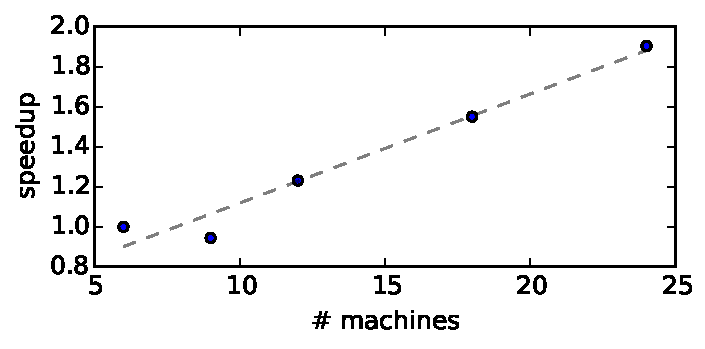
\includegraphics[width=0.6\columnwidth]{imgs/linear-speedup}
%      \caption{Linear speedup when increasing computing resources.}
%   \label{fig:scalability}
% \end{figure}

% We first run a scale-out experiment to determine how our implementation scales with increasing cluster resources. We use the \textit{mnist8m} dataset with 8 million observations, consisting of 784 features each, giving us a matrix with more than $6$ billion cells as input data. We run our spark implementation of Algorithm~\ref{alg:dskl_svm_distributed} on this dataset on a cluster comprised of 24 machines and choose the sample sizes in a way that the aggregate sample size amounts to the full dataset. We start by leveraging 6 machines and subsequently increase this number to 9, 12, 18 and the full 24 machines. We measure the runtime for each subsequent run; On the full cluster, an iteration takes approximately 6 seconds\footnote{note that our implementation is a proof of concept in Scala; there is much rooom for performance improvements by using a language like C++ and native matrix libraries; furthermore, the runtime is dependent on the number of samples drawn}; We compute the speedups in comparison to the smallest setup (c.f.,~Figure~\ref{fig:scalability}) and find that increasing the cluster resources results in a roughly linear speedup. Although the speedups are far from perfect, mostly due to the costly broadcast operation, our algorithm shows the desired scalability property: the ability to handle more data by simply increasing cluster resources.

\section{Conclusion}
When modelling complex functions, the practitioner usually has three main options: Decision-Tree based methods, Neural Networks and Kernel methods. Decision Tree based methods appear to dominate most Kaggle competitions and in general have a stunning performance on real-world data sets \cite{Caruana2006}. But when a modelling task goes beyond simple supervised settings, these methods might not be the first choice. Deep neural networks yield large performance improvements on many tasks and are successfully used for unsupervised learning as well -- but they can be difficult to design and train. 
This is where kernel methods offer some advantages: Instead of optimizing a network architecture one simply picks an off-the-shelf kernel function for a given type of data and then one performs model selection over just a handful of kernel parameters for both unsupervised and supervised learning in a principled manner.

We have proposed a very simple algorithm for scaling up kernel learning that is easy to implement and parallelize. Our results demonstrate that the proposed method achieves competitive performance on standard benchmarks. We hope complementing the existing methods for large scale kernel learning as well as other successful methods such as random forests and neural networks will ultimately help to understand better the strengths of the respective methods, independent of factors such as hardware and optimization procedures. 

%One reason for the success of neural networks was the availability of new hardware for training them. This technology can be beneficial for other learning paradigms as well, including the approach presented here. A direction of future research is to speed up the parallel implementation using graphics cards. 

Our experiments on artificial data showed that there are conditions under which the explicit kernel map approximation approach performs worse than the empirical kernel map, in agreement with previous results in \cite{Vedaldi2010}. But a direct comparison of the presented approach with results obtained with explicit kernel maps as in \cite{Dai2014} is difficult, due to the differences in the implementations. An important topic of future research will be to investigate when explicit kernel map approximations as in \cite{Rahimi2008, Dai2014} should be preferred over the empirical kernel map approaches presented here. However in terms of implementation applying the doubly stochastic empirical kernel map approach to more complex kernels could be considered simpler than implementing a dedicated explicit kernel map as in \cite{Dai2014} for every kernel function. 

We found that in its presented form, our approach is not well suited for distributed data processing systems like \textit{Apache Spark}~\cite{Zaharia2012} or \textit{Apache Flink}~\cite{Alexandrov2014} which use a shared-nothing architecture. This is due to the fact that a naive distributed execution of our algorithm would impose a high amount of communication per iteration for aggregating the gradients over the network, as well as for re-distributing the updated parameter vector. A variant that updates parameters locally on the slaves in the cluster, and only updates the global model from time to time (thereby reducing inter-machine communication) could be worth to look into in the future. Another interesting direction would be implement the doubly stochastic approach on graphics cards, to leverage their potential for massive parallel computation, which our algorithm amends itself to.

\newpage

{\small
  \bibliography{dskl}
  \bibliographystyle{plain}}

\end{document} 
